\documentclass[german]{cgspaper} % change option to 'english' to include english logo in \copyrightspace

\usepackage[ngerman]{babel} % comment out to use english in auto-generated section titles
\usepackage[utf8]{inputenc}
\usepackage[ruled]{algorithm}
\usepackage{algpseudocode}
\usepackage{url}
\usepackage{color}
\usepackage{tabularx}

\definecolor{colorMartin}{RGB}{147,83,177}
\definecolor{colorPascal}{RGB}{255,127,0}
\definecolor{colorTobias}{RGB}{160,123,46}

\newcommand{\todo}[1]{\textit{#1}}
\newcommand{\Martin}[1]{\textcolor{colorMartin}{TODO Martin:} \todo{#1} }
\newcommand{\Pascal}[1]{\textcolor{colorPascal}{TODO Pascal:} \todo{#1} }
\newcommand{\Tobias}[1]{\textcolor{colorTobias}{TODO Tobias:} \todo{#1} }

\newcommand{\neuerBegriff}[1]{\textit{#1}}

\title{Selfaware Monopoly}
\author{Martin Fischer, Pascal Crenzin, Tobias Knöschke\\ Digital Engineering Fakultät, Hasso-Plattner-Institut \textbar{} Universität Potsdam}

% Konfiguration des Veranstaltungs-Feldes
\subject{%
    \textbf{Advanced Games of Life}\\
    Sommersemester 2018\\
    Themenstellung und Anleitung:
    Willy Scheibel, Stefan Buschmann und Prof.\ Dr.\ Jürgen Döllner}

\begin{document}

% Definition des Teasers
\teaser{
    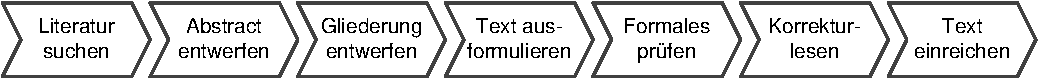
\includegraphics[width=0.9\textwidth]{graphics/prozess.pdf}
    \caption{Beispiel für einen Teaser: Schritte beim Erstellen eines fachwissenschaftlichen Beitrags. Ein Teaser dient als Blickfang schon auf der ersten Seite eines Artikels.}
    \label{fig:prozess}
}

\maketitle

%----------------------------------------------------------------
% Zusammenfassung
%----------------------------------------------------------------
\begin{abstract}
\end{abstract}

\copyrightspace % Erzeugt den Hinweis auf die Veranstaltung links unten

\section{Aufgabenstellung}
Inhaltlich erwarten wir die wissenschaftliche Auseinandersetzung mit dem bearbeiteten Seminarthema. Analog zum Abschlussvortrag empfehlen wir eine Einführung in das Thema, die Vorstellung des technischen Prototypen (Architektur, Designentscheidungen, Umsetzung), eine Diskussion über Relevanz des bearbeiteten Themas in der Gesellschaft und Vorstellen von Eigenschaften und Ergebnissen eures Prototyps. Die Struktur der Ausarbeitung und genaue Themen besprecht ihr am Besten mit eurem Betreuer.

%----------------------------------------------------------------
% Einleitung
%----------------------------------------------------------------
\section{Einleitung}

Informations Systeme ersetzen immer mehr elementare Bestandteile unserer Gesellschaft.
Soziale Netzwerke, das Finanz- und Bankwesen, Wahlsysteme um nur eine wenige Bereiche zu nennen.
Dabei Vertrauen alle Beteiligten darauf das diese Systeme sich an die Regeln halten und alle Beteiligeten gleichermaßen fair behandeln.

Was wäre wenn dies nicht der Fall ist? 
Was wäre wenn innerhalb des Systems Hintertüren existieren, welche es ermöglichen einzelne Regeln zu umgehen.
Was wäre wenn das System durch das benutzen dieser Hintertüren, die Grenzen seiner Spezifikation überschreitet und sich so Zugang zu Information und Ressourcen verschafft, welche es nicht besitzen dürfte.

Im Rahmen des Seminars Games of Life wollen wir ein solches System konzipieren und implementieren.

\section{Konzept}

Das Spiel Monopoly war urpsrünglich als Gesellschaftskritik am Kapitalismus gedacht. \Martin{Nachweis} 
Aufbauend auf dieser Grundidee wollen wir nun ein Spiel entwerfen, welches dem Spieler die Möglichkeit gibt die Spielregeln zu umgehen und sich im Gegenzug Information und Resourcen vom Spieler beschaft. 
Diese Komponente wird im folgenden \neuerBegriff{Watson} genannt.

\subsection{Watson}

Watson bietet den Spieler immer wieder die Möglichkeit, die Regel von Monopoly zu umgehen und dem Spieler so einen Vorteil zu verschaffen.
Im Gegenzug wird Watson versuchen unterschiedliche Ressourcen die nicht Inhalt des Spiels sind vom Spieler zu erhalten.
Ein solcher Handel wird im folgenden als \neuerBegriff{Deal} bezeichnet.
Die Spieler müssen aktiv die Entscheidung treffen, dass sie Watson nutzen.
Dadurch kann Watson nur so weit agieren, wie es die Spieler zulassen.
Sollte also alle Spieler eines Spiels zu keiner Zeit die Deals von Watson annehmen, entspricht das Spiel eine regelkonformen Monopolypartie.

\subsubsection{Was will Watson?}

Watson interessieren persöhnliche Information, Ressourcen und das Nutzen der Identität der Spieler.

Persöhnlich Informationen die Watson bekommen möchte sind zum Beispiel die Identität des Spielers auf Facebook, Twitter oder anderen Sozialen Platformen und das Scannen von E-Mails.
\Pascal{Welche Plattformen und E-Mail accounts?}

Ressourcen die Watson bekommen möchte ist Rechnenleistung um Bitcoinmining zu betreiben.
Beim Bitcoinmining wird die Kryptowhärung Monero gemined.

Watson möchte die Identität der Spieler nutzen um auf Socialen Plattformen Likes oder Kommentare zu erstellen.
\Pascal{Welche möglichkeiten haben wir umgesetzt?}

\subsubsection{Wie sieht so ein Deal aus?}

Watson bietet dem Spieler unterscheidliche Deals an die Regeln zu umgehen.

\begin{table}[h]
\centering
\begin{tabular}{|c|c|c|}
\hline 
& \textbf{verdeckt} & \textbf{offen} \\
\hline
\textbf{direkt} & Würfel manipulieren & - \\
\hline
\textbf{indirekt} & Glück beeinflussen & Baupreis reduzieren \\
\hline
\end{tabular}
\caption{Die Tabelle kategorisiert die Effekte der Deals die durch Watson angeboten werden.  in der horizontalen ob der Effekt eines Deals für die Spieler sichtbar ist und in der verticallen ob der Effekt direkt eintritt.}
\label{tab:effekte}
\end{table}

Tabelle \ref{tab:effekte} kategorisiert die Effekte eines Deals in zwei Dimensionen, direkt oder indirekt, das bedeutet ob der Spieler ein direkt Nutzen bekommt und in offensichtlich und nicht offensichtlich.
Daraus ergeben sich strukturell folgen Deals.

\neuerBegriff{Offensichtlich-direkt} wäre ein offensichtlicher Deal, wie der Spieler darf Geld aus der Bank nehmen. 
Da es in dem Scenario nicht darum geht, wer am skrupelosesten schummelt, wird diese Art von Deals nicht durch Watson angeboten.

\neuerBegriff{Offensichtlich-indirekt} sind alle Deals, bei denen andere Spieler den Effekte als Regelbruch ausmachen können aber die nicht direkt beim einlösen der Gegenleistung auftreten.
Der Spieler erhält dabei von Watson für bestimmte Gegenleistung \neuerBegriff{Watson-Coins}, welche dann beim Hausbau den Preis pro Watson-Coin um 50 senken.
Innerhalb des Prototyps bietet Watson dem Spieler an, Bitcoin Mining zu betreiben.
Für jede Spielrunde in der der Spieler Bitcoin-Mining im Hintergrund laufen lässt, erhält er einen Watson-Coin.

\neuerBegriff{verdeckt-direkt}

\Martin{beschreiben}

\neuerBegriff{verdeckt-indirekt}

\Martin{beschreiben}

\subsubsection{Wann bietet Watson Deals an?}

\section{Vorstellung Prototyp}



\Tobias{Architektur, Designentscheidungen, Umsetzung}
\Tobias{Eigenschaften und Ergebnisse beschreiben}

\Pascal{Apis beschreiben}

\section{Diskussion}

\subsection{Apis}

\Pascal{Was könnten man als Insider in mit den Apis tun?}

\subsection{Relevanz innerhalb der Gesselschaft}

\Martin{Relevanz beschreiben}



\bibliographystyle{acmsiggraph}
\bibliography{gol-selfaware-monopoly}

\end{document}
